% !TEX root = ../main.tex
\section{What makes the recipe work?}
\label{sec:analysis}
\subsection{Prompt imitation and downstream adaptation}
\begin{figure}[t]
\centering
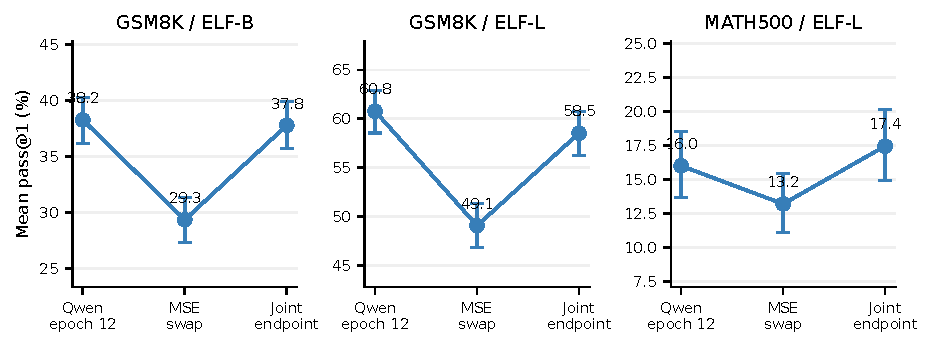
\includegraphics[width=\linewidth]{figures/prompt_stages.pdf}
\caption{Prompt substitution and subsequent adaptation at 32 steps. Each point averages four matched seeds; bars show 95\% problem-bootstrap intervals. The first two conditions share the same epoch-12 ELF weights. Later joint training updates both ELF and the prompt encoder.}
\label{fig:prompt}
\end{figure}
Replacing teacher prompt states with an MSE-trained encoder causes an immediate accuracy loss (Figure~\ref{fig:prompt}). For GSM8K ELF-B, the drop is 38.25\% to 29.34\%; for ELF-L, 60.78\% to 49.07\%; for MATH ELF-L, 16.00\% to 13.20\%. These losses remain after selecting the better-fitted prompt EMA $0.999$, rather than the more slowly adapting $0.9999$ state. Prompt MSE alone therefore does not capture all the properties of conditioning needed by the denoiser.

Subsequent joint training recovers 8.43, 9.46, and 4.25 percentage points, respectively. The final accuracies are 37.77\%, 58.53\%, and 17.45\%. These 32-step, four-seed values are specific to the stage ablation and differ from the 64-step headline evaluation. Because both models adapt after the swap, recovery measures the complete training stage rather than prompt-only improvement. Appendix~\ref{app:prompt} gives paired intervals and prompt-MSE curves.

The early joint-training control in Figure~\ref{fig:fourarm} complements the prompt-swap experiment. In these two-seed learning curves with shared $t=\tau^2$ inference, the random-joint arm reaches 3.98\%, 7.77\%, and 8.61\% at epochs 2, 4, and 6, versus 12.40\%, 26.61\%, and 31.01\% for teacher-prompt training. The four-seed epoch-six evaluation in Table~\ref{tab:representation} confirms this large gap. Within this six-epoch budget, supplying a stable contextual prompt representation is substantially more effective than learning both components from the beginning.

\subsection{Asynchronous clocks and common time warps}
% !TEX root = ../main.tex
\begin{table}[t]
\caption{Four-seed ELF-L schedule comparison at 32 steps (42/123/456/789). Entries are mean pass@1 (\%). Epoch 21 uses ELF/prompt EMA $0.9999/0.9999$; NFT uses $0.99/0.99$ at GSM8K update 500 and MATH update 600. MATH uses Math-Verify.}
\label{tab:schedules}
\centering\small
\setlength{\tabcolsep}{4pt}
\begin{tabular}{lrrrr}
\toprule
Layer clocks & GSM8K e21 & GSM8K NFT & MATH e21 & MATH NFT \\
\midrule
$(1.5,1.5,1.5)$ & 57.18 & 62.77 & 17.90 & 24.05 \\
$(2,2,2)$ & 57.39 & 62.57 & 17.35 & 22.30 \\
$(2.5,2,1.5)$ & 58.53 & 62.34 & 17.45 & 22.95 \\
\bottomrule
\end{tabular}
\end{table}

Layer-specific clocks change both where the model is queried and how each latent group advances. A useful control therefore includes synchronous $(2,2,2)$, not only the identity schedule $(1,1,1)$. We also compare common exponents 1.5 and 2.5 and the reversed assignment $(1.5,2,2.5)$.

Table~\ref{tab:schedules} compares the headline allocation with shared exponents 1.5 and 2 using four seeds. At GSM8K epoch 21, async improves over $(2,2,2)$ by 1.14 points, with paired 95\% interval $[0.45,1.82]$, and over $(1.5,1.5,1.5)$ by 1.35 points, $[0.53,2.14]$. For the other three endpoints, all paired pass@1 intervals against these controls include zero. The MATH NFT gain over $(2,2,2)$ is 0.65 points, $[-0.60,1.85]$; a shared exponent of 1.5 has the higher point estimate. Thus the gains from layer-specific clocks depend on the checkpoint. Appendix~\ref{app:schedules} retains the broader two-seed sweep. We retain the fixed asynchronous allocation for the headline reasoning endpoints and use shared $t^2$ specifically for the four-arm early-training controls.

\subsection{More denoising steps or more answers?}
\label{sec:budget}
For $k$ samples with $S$ denoising steps each, define the transparent compute proxy $B=kS$. At each of the six pre-/post-NFT endpoints, the 8-, 16-, 32-, and 64-step cohorts contain 64, 32, 16, and 8 samples per problem, respectively, so every depth reaches $B=512$. Oracle pass@$k$ counts a problem as solved if a correct answer appears anywhere among the samples. Voting groups equivalent final answers without consulting the reference and selects the largest group. We average uniformly over tied winning groups.

\begin{figure}[t]
\centering
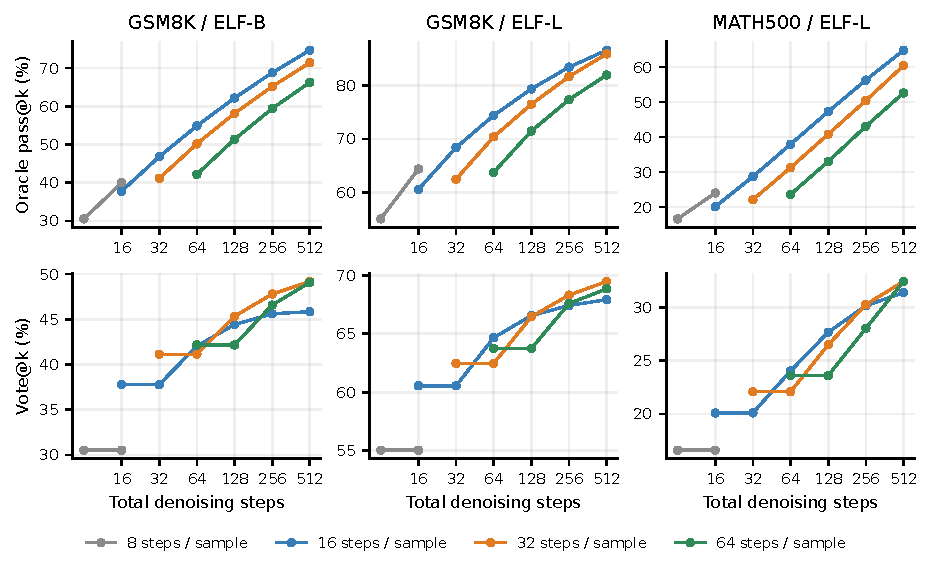
\includegraphics[width=\linewidth]{figures/nft_budget.pdf}
\caption{Inference allocation after NFT. Horizontal axes show total denoising steps $kS$. Top: oracle pass@$k$; bottom: final-answer voting. All four depths reach 512 total steps, including 8 steps with 64 samples. Markers correspond to powers-of-two sample counts. Short trajectories increase oracle coverage, while answer voting favors longer trajectories at this budget.}
\label{fig:budget}
\end{figure}

At $B=512$, 8 steps with 64 samples gives the highest observed oracle accuracy at all three NFT endpoints: 76.04\% on GSM8K ELF-B, 88.78\% on GSM8K ELF-L, and 67.00\% on MATH. Across both training stages, it leads at five of six endpoints; pre-NFT ELF-B is one problem behind $16\!\times\!32$. Yet $8\!\times\!64$ has the lowest voting accuracy at all six endpoints. For MATH after NFT, oracle accuracy is 67.00\% with $8\!\times\!64$, versus 60.40\% with $32\!\times\!16$, while voting reverses the preference: 25.79\% versus 32.41\%. Table~\ref{tab:budget512} gives all allocations. These point estimates distinguish covering more problems with at least one correct sample from reliably selecting a correct answer.

The step proxy omits repeated prompt encoding and terminal decoding. We preserve steps as the primary horizontal axis and separately plot measured time against total steps (Appendix~\ref{app:cost}). At $B=512$, MATH NFT inference costs are 6.32, 5.75, 5.45, and 5.33 amortized H200 seconds per problem for $8\!\times\!64$, $16\!\times\!32$, $32\!\times\!16$, and $64\!\times\!8$, respectively. Extra samples introduce overhead even when total denoising steps are fixed.

\subsection{NFT improves correctness while concentrating answers}
\label{sec:diversity}
To compare stages without changing sample count, we analyze eight matched draws at 32 steps. NFT reduces the mean number of distinct answers from 4.18 to 3.67 for GSM8K ELF-B, from 3.10 to 2.55 for GSM8K ELF-L, and from 5.91 to 5.48 for MATH. Pairwise answer agreement increases in all three settings.

For GSM8K, gains in pass@1 coexist with small changes in oracle pass@8: $+1.06$ points for ELF-B and $+0.68$ for ELF-L, with paired intervals that include zero. MATH gains $4.40$ points in oracle pass@8 and $6.89$ in vote@8, with intervals $[0.60,8.20]$ and $[4.11,9.69]$. These results distinguish concentrating probability on existing successes from expanding coverage. Appendix~\ref{app:diversity} includes per-problem coverage transitions, subject/difficulty breakdowns, and the NFT group-discard diagnostic.
